\documentclass[12pt,a4paper,bibliography=totocnumbered]{scrartcl}
\usepackage[utf8]{inputenc}
\usepackage[USenglish]{babel}
\usepackage{booktabs}
\linespread{1.25}
\usepackage[T1]{fontenc}
\usepackage{amsmath,amssymb,amstext}
\usepackage{graphicx}
\usepackage{fancyhdr}
\usepackage{titling}
\usepackage{color}
\usepackage{array}
\usepackage{chemmacros}
\usepackage{float}
\usepackage{chemexec}     
\usepackage{chemfig,chemnum}
\usepackage{natbib} 
\usepackage[hyphens,spaces]{url}
\newcolumntype{M}[1]{>{\centering\arraybackslash}m{#1}}
\usepackage{multirow}
\setlength{\parindent}{0em} 

%\addbibresource{literatur.bib}


\begin{document}
	
	
	\thispagestyle{empty}
\setlength\droptitle {-20.5mm}
\renewcommand{\maketitlehooka}{
	\includegraphics[width=\linewidth]{{picture/HUlogo.png}}\par\vskip 0.7cm}
\title{\normalsize \textbf{LEBENSWISSENSCHAFTLICHE FAKULTÄT\\ INSTITUT FÜR BIOLOGIE} \vspace*{1.5cm}
 \\ \Large \vspace*{15pt} \textbf{BACHELORARBEIT}\\ \large \textbf{ ZUM ERWERB DES AKADEMISCHEN GRADES} \\ \textbf{BACHELOR OF SCIENCE} \\ \vspace*{1.5cm} "Strukurelle Analyse eines kombinierten Models zur osmotischen Stressantwort in Hefe"\\ \vspace{0.2cm} "Structural analysis of a combined model for an osmotic stress response in yeast" \\ \vspace*{1.5cm} \normalsize vorgelegt von \vspace*{0.3cm} \\ Jan Piotraschke\\ geb. am 28.08.1993 in Hamburg \vspace*{1.2cm} \\angefertigt in der Arbeitsgruppe Biophysik \\am Institut für Biologie \\ \vspace*{1.2cm}Berlin, der 17. Januar 2019 \vspace*{-0.7cm}  }

\date{}
\bibliographystyle{unsrt}
%\cfoot{\thepage}

\maketitle
\textcolor{white}{}
\newpage



	\section{Zusammenfassung}
\pagenumbering{Roman} 
Um besser das Zusammenspiel zwischen dem Zellvolumen der Hefe Saccharomyces cerevisiae, wenn diese hyperosmotischen extrazellulären Stress ausgesetzt ist, und der damit verbunden HOG MAPK Signalweg bzw. Plasmamembran-Ionentransport Regulierung zu verstehen, haben wir dafür ein mathematisches Model aus ODEs und algebraischen Gleichungen konstruiert. Dies geschah durch zusammenfügen von drei getesten Einzelmodellen.\\
Dafür haben wir einen neuartigen Simulationsansatz in Python3 Code mit Hilfe einer lokalen Datenbank implementiert.\\
Das kombinierte Model verdeutlicht die wechselseitigen Abhängigkeiten zwischen dem Hog Signalweg, der Volumenregulation und der extra-/intrazellulären Ionenkonzentrationen.

\section{Abstract}
To better understand the interplay between the cell volume of the yeast Saccharomyces cerevisiae when faced with hyperosmotic extracellular stress and the corresponding regulation of the HOG MAPK signaling pathway and the plasma membrane ion transport, we constructed a mathematical model by merging three tested single models. The mathematical model consists out of ODEs and algebraic equations. \\
For this, a novel simulation approach in python3 code with the help of a local database was implemented.\\
The combined model clarifies the dependencies between the hog pathway, the volume regulation and the extra-/ intracellular ion concentrations. 


\newpage	
	\tableofcontents \thispagestyle{empty} \newpage
\pagenumbering{arabic} 
\setcounter{page}{1}
	% \cfoot[{\thepage\ of \pageref*{LastPage}}]{\thepage\ of \pageref*{LastPage}} 
\section{Introduction}
\pagestyle{headings}


\subsection{system biology}
System biology is there for the extraction of a system wide understanding of living organismen. This includes the interaction of multiple proteins, genes, metabolits et cetera, which are measured in the laboratory. This approach gets more significant in the analysis of executed omics experiments which easily results in data in the gigabyte range (Zitieren: Toward an integrated ...). Mathematical modeling has proven to be a promising tool for the study of the complex processes of environmental stress adaptation, to reveal the role of each biological component in the system and to reveal  how the system level properties emerged from collected activites of individual components \cite{Ke_2013}. \\\\
Currently limitations of the system biology approach are the usages and constructions of mathematical equations which should represent the biological system. This is a trade off between reduction of the system of interest without dimishing the quality of the information value or reasonableness intended digital twin. Another important problem is that there does not exists a complete biological understanding and knowledge of all system component. The system biological appproach is therefore only a heuristic approach (zitieren!!!) \\\\
In-depth insights of an investigated system are e.g. useful for medicine and the biotechnology sector (cite: Toward an integrated software platform for systems pharmacology!!!!) because this results in the improvement of  
well constructed mathematical models of a cell system could be useful for the design of target-oriented medications. \\\\
An increase in external osmolarity leads to a cell volume reduction. The cell counteract this high osmotic pressure by increased intracellular glycerol as an osmolyte and restores in this way its volume. \\


Mathematical models \textit{in silico} are further helpful to test laboratory experiments \textit{in silico} to identify meaningful experiments by construction of DoE (Design of Experiment). This helps to save the resources (e.g. money, time) of the experimentalist and could results in a deeper understanding of the underlying biological system.\\\\

\subsection{Saccharomyces cerevisiae}
The yeast Saccharomyces cerevisiae (\emph{S. cerevisiae}) is a unicellular eucaryotic organism and belongs to the class of fungi \cite{Feyder2015}. It was the first eucaryotic organism where the whole genome had been full sequenced. \cite{goffeau1996life}. \emph{S. cerevisiae} is one of the beast characterized eukaryotic models \cite{Feyder2015}.\\\\
In nature, the environment of S. cerevisiae varies in factors like temperatur, nutrient levels or osmolarity with the time and the cell must adapt with these changes. \cite{JannisUhlendorf} The Hog-Pahtway in yeast has a significant role in the adaption process after an osmotic stress exposure. It normalize the volume of the cell and with that the water balance with an accumulation of the osmolyt glycerol inside, by closing the glycerol membran transporter Fps1 (\cite{Saito2012},  \cite{ASimpleMathematicalModel}) and the production of glycerol.  

\subsection{state of the art}
It already exists multiple models for the hog pathway (signaling module), ion transport (transport module) and the volume regulation (volume module) (!!! alles hier noch mit Zitaten belegen). The signaling module keeps tracks of the stress response signaling pathways \\
Each of these models describe a part of the cell system while assuming other important aspects of the system as constant (see picture \ref{IntersectionsOfTheModels}).

\begin{figure}[h!]
	\begin{center}
		\begin{minipage}{0,8\textwidth}
			
			\includegraphics[width=\textwidth]{picture/model_intersections.png}
			\caption{intersections of the three models } 
			\label{IntersectionsOfTheModels} 
		\end{minipage}
	\end{center}
\end{figure}

In our momentan state of knowledge, there is not yet a model which integrate this three modules into a single model. The combined model simulates the interaction between extra- and intracellular ionconcentration, changes in cell volume and the activity of the MAP cascade (???). The model senses the differences in the osmolarity between the cell and its environment and adapt with the important high osmolarity glycerol (HOG) signaling pathway with the MAP cascade the cell volume and the intracellular osmolyt concentrations. 

\subsection{theory of the used models}
\subsubsection{ion model}
Per diffiniton, osmolarity means the amount of substance $n$ of osmotic activ particles per volume $V$ of the solution. Osmotic pressure accurs if two solutions with different osmolarity are seperated by a semipermeable membrane, where not all substances can pass the membrane for creating an equilibrium.\\
S. cerevisiae has a plasma membrane which functions as a semipermeable membrane. Water can diffuse freely through it, to adapt to the osmotic changes. At a hyperosmotic shock in the extracellular environment, water will flow out of the cell and let the cell shrink in volume. Cause of the shock event the high osmolarity glycerol (HOG) pathway in S. cerevisiae gets activ and synthesis the osmolyte glycerol. With that the cell increases the internal osmolarity and restores it’s volume cause of the influx of water.\\\\
The immediate effect on yeast to an osmotic shock involves water outflow and decreasing volume \cite{ASimpleMathematicalModel}.\\
The ion model consists out of a non-equivilibrium thermodynamic (NET) approach to model the transport of the ion over the plasma membrane. NET is the analysis of spartial inhomogeneous systems and of time dependent processes. It is not valid if there are very fast processes or big inhomogeneity. The ion model assumes that both compartimens are well mixed. This way the NET approach hold true. \\
Fluxes over membranes are irreversible processes. This will lead to a production of entropy in the system, which is calculated by the entropy production density $\sigma$ which is respresented with the equation \ref{EntropyProductionDensity}

\begin{equation}\label{EntropyProductionDensity}
	\sigma = \vec{J_Q}\left(\frac{1}{T}\right) - \sum_{i=1}^{k}\vec{J_{c_i}}grad \left(\frac{\eta _i}{T}\right) + \sum_{r=1}^{R}J_r \frac{A_r}{T} \geq 0
\end{equation}
Equation \ref{EntropyProductionDensity} summeries the production of entropy under the conditions of temperatur difference, concentration difference and chemical reactions.
Fundamentally, $\sigma$ can only be created by fluxes $J$ with it’s forces $X$. In the area around equilibrium we can further assume that a flux $J$ is linearly coupled over a phenomenological coefficient $L$ with it’s forces $X$, because at equilibrium all forces and fluxes vanish. Under this condition the following statement holds true.
\begin{equation}\label{stoeachimetricCoeff}
	\sigma = \sum_{i}J_i X_i =\sum_{i}\sum_{j}L_{ij}X_j X_i
\end{equation}
After some other assumption made from the ion model (for deeper insight see \cite{Gerber_2016}), the equation for the flux of ion k is:
\begin{equation*}
J_k = \sum_{j=1}^n L_{kj}(RT\cdot ln\left(\frac{c_k^{in}}{c_k^{out}}\right) + z_kF\Delta \phi ) + L_{kAr}A_{Ar}
\end{equation*}
In the ion model a glycerol stimulus is further simulated. Ion regulation determines many physiological parameters, such as cell volume \cite{Ke_2013}.\\\\
\subsubsection{volume model}
Turgor pressure prevents exaggerated swelling and maintains cell shape \cite{volumeModel}. The volume model \cite{volumeModel} describes the water flux $J_w$ between the cell and the environment with 
\begin{equation}\label{waterFlux}
	J_{w} = - \frac{d}{dt} V_{os} = G * Lp * (\pi_e + \pi_t - \pi_i)
\end{equation}
with $Lp$ as the hydraulic conductivity, $G$ the cell surface and the internal, external and turgor pressure  ($\pi_i$, $\pi_e$ , $\pi_t$). The volume model only holds true for a individual yeast cell in G1 phase \cite{volumeModel}.
The cell volume depends essential on the relation of the internal, external and turgor pressure. The internal and external pressure $\pi$ depends on the concentration $c$ of the osmotic active substance in the corresponding areas correlated over the equation \ref{osmotic_pressure}
\begin{equation} \label{osmotic_pressure}
	\pi = c \cdot R \cdot T	
\end{equation} 

\subsubsection{hog model}
The hog model is composed out of the Hog1 Mitogen Activated Protein Kinase (MAPK) cascade. This cascade is conserved even in higher eukaryotes including humans (\cite{ASimpleMathematicalModel}). The Hog1 MAPK is activated in the response to an increase in extracellular osmolarity \cite{Saito2012}. All other non-osmotic stresses (e.g. temperature stres \cite{Saito2012}) which are known to also activate the HOG pathway are not represented in this model. The MAPK pathways are important for transmitting and processing signals from the cell membran into the cell \cite{ASimpleMathematicalModel}. \\
Hog1n MAPK is activated by the upstream Pbs2 MAP kinase kinase (MAPKK) by phosphorylation. 


\newpage
	\section{material and methods}
\subsection{software development}
Cause a simulation for the combined models could take several minutes and the thereafter calculation and handling of this results are not garanted to work in the process of a program development, I came up with the idea that the results must be safed after each simulation and the analysis of them should be run in another program, as 
\begin{center}
	first program : simulation --> save data\\
	second program : data --> analysis
\end{center}
For the construction of this workflow I implemented a database and connected it to my python script. For the storing logic of the data I used a concept from CDISC for clinical trials which allowed me to construct the useful column names, data types and table in the database. Because a simulation of ODEs and algebraic equations can have pending sets of initial values, parameter values or equations terms, I expanded the concept of CDISC to the area of system biology and designed new data storage procedures. In picture (!!! Bild zeichnen lassen und hier einfügen) you can see  the proposed workflow. \\ The intention for the  implementation of CDISC to system biology was the fact, that the FDA is moving towards CDISC standards for regulatory submissions \cite{SDTMStandard}.\\\\
With this approach, we can analysis and try new codes snippets with the results of a long simulation in seconds. \\
A version control mechanismen in the context of model construction was implemented with the help of a local database. The whole software development framework is visualized in (hier das Bild einfügen !!!!!!!!). \\\\
Furthermore, the storage of the model in a JSON file was in this way designed, that a natively typed equation in a .txt file format like 
\begin{equation*}
	\frac{d}{dt} Na_{in} = \frac{J_{Na} \cdot G}{V_{os}} \cdot 10^6 - Na_{in} \cdot V_{ratio} 
\end{equation*}
gets automatically seperated in the terms $\frac{J_{Na} \cdot G}{V_{os}} \cdot 10^6$ and $- Na_{in} \cdot V_{ratio}$. This allowes us to simulate each term component and analyse its constribution to the result of the equation in relation to the time.\\
\newpage
	\section{Results}
\subsection{results of single models}
Before merging the three models together it must be controlled whether each model is implemented correctly for itself. The pictures of the models simulation results are the guide for this. Sometimes there are discrepanies between the puplished model and the picture which should represent the model.  Hereafter, the implementation process for each of the models is described.\\
To better retrace the implementation steps it is recommended to read the paper for the hog \cite{Zi_2010}, ion \cite{Gerber_2016} and volume model  \cite{volumeModel}.

\subsubsection{Ion model}
The challenges with the implementation of the ion model were, that the presented equations, initial values and parameters did not result in the intended system behaviour. \\
After an in-depth analysis of the equation there were two anomalies:

\begin{enumerate}
	\item the calculation of the change of the inner proton ion concentration has \emph{Bf} as an undefined parameter
	\item the fluxes have the wrong units
\end{enumerate}

For solving the problem with the undefined parameter the ODE was constructed by deriving the formula for the calculation of the pH value for diluted solution equation \ref{pHforDilution}
\begin{equation*}
	pH = - log_{10}([H^+])\\
\end{equation*}
\begin{equation}\label{pHforDilution}
	\frac{d}{dt}pH = \frac{d}{dt}(-log_{10}([H^+])) = - \frac{1}{ln(10)} \frac{d}{dt}ln([H^+]) = - \frac{1}{ln(10)}\frac{1}{H^+} \frac{dH^+}{dt}
\end{equation}
and combine it with the equation \ref{pHchange} for the change of the pH Value as a result of proton flux (\cite{martinafroehlich})
\begin{equation}\label{pHchange}
	\frac{d}{dt}pH_{in} = \frac{J_H \cdot Surface}{V_{in} \cdot pbc}
\end{equation}
	
The equation \ref{usedProtonFlux} 
\begin{equation}\label{usedProtonFlux}
- \frac{1}{ln(10)} \frac{1}{H^+}\frac{dH^+}{dt} = \frac{J_H \cdot Surface}{V_{in} \cdot pbc}\\
\Rightarrow \frac{dH^+}{dt}=-\frac{J_H \cdot Surface \cdot ln(10) \cdot H^+}{V_{in} \cdot pbc}
\end{equation}

was used for modelling the change of the inner proton concentration. $pbc$ is the proton buffer capacity.\\\\
To solve the problem with the wrong units it was identified, that the equation for the reported fluxes only missed the unit Kelvin ($K$) in its numerator. Multiplying the equation with the temperature $T$ solved this problem and resulted in the equation \ref{IonFlux}.
This model represents the model with the initial values and global quantities and volumes from Table 4 in the ion paper \cite{Gerber_2016}. The phenomenological and stoichiometric coefficients were adopted from the original Copasi ion model file. In picture \ref{IonImplemented} the implemented ion model is visualized.
\begin{figure}[htbp]
	
	\begin{minipage}{0,5\textwidth}
		
		\includegraphics[width=\textwidth]{picture/Ion_Paper.png}
		
		\label{IonPaper} 
	\end{minipage}
	\begin{minipage}{0,5\textwidth}
		
		\includegraphics[width=\textwidth]{picture/ion_examine.png}
		
		\label{IonImplemented} 
	\end{minipage}
	\caption{left: membrane voltage in the ion paper for different NaCl stimulus (0.01 mM - 10 mM); right: the simulated implemented ion model for the same stimulus range }
\end{figure}


\subsubsection{hog model}
For the implemtation of the hog model, the \textit{Table S1-S3} and the Matlab code for the used $NaCl$ impulse in \textit{Code S1 } in the supporting informations of the paper were implemented in the python3 environment. No difficulties were encountered. The only problems occur with the handling of the intended stimulus time length.

\begin{figure}[htbp]
	
	\begin{minipage}{0,5\textwidth}
		
		\includegraphics[width=\textwidth]{picture/Hog_Paper.png}
		
		\label{hogPaper} 
	\end{minipage}
	\begin{minipage}{0,5\textwidth}
		
		\includegraphics[width=\textwidth]{picture/hog_examine.png}
		
		\label{hogImplemented} 
	\end{minipage}
	\caption{}
\end{figure}

\subsubsection{volume model}
The volume model could not be implemented with only the corresponding paper because the model wants to describes the change of the non-osmolytic volume $V_b$ but missed to note down an equation for this.\\
After consultation with my supervisior and one of the author of the model about this information gap, it was recommended that I use the already implemented volume model in their local network "YCM" as a template. After translating this template in my own software structure, no problems were encountered. In the appendix I documented the used ODE, algebraic equation, parameter and initial values for this model. 
% schritte der volume model implementierung
\begin{figure}[htbp]
	
	\begin{minipage}{0,5\textwidth}
		
		\includegraphics[width=\textwidth]{picture/Volume_Paper.png}
		
		\label{volumePaper} 
	\end{minipage}
	\begin{minipage}{0,5\textwidth}
		
		\includegraphics[width=\textwidth]{picture/volume_examine.png}
		
		\label{volumeImplemented} 
	\end{minipage}
	\caption{}
\end{figure}


\subsection{merging of the models}
The process of merging models is a tricky task. There exists some good guideline \cite{Liebermeister2008ValidityAC} for this.
Hereafter, the used essential steps are sketched:
\begin{enumerate}
	\item equations: One of the first steps in the process of model merging is to control whether there is a conflict between assumptions of the description of the biological systems. Conflicts must be resolved by combining equation terms or discard some informations
	\item names: Find all the overlaps in the variable and parameter naming and convert them to a common sets of names
	\item units: Standardize all used units for the parameter and initial values to a common set. In this process new factors where give to individual values if the unit changes requires that.
\end{enumerate}
Changes in the equation design (ODE and algebraic equation) were done in the process of merging the models and are presented below:

\begin{table} [h]
	\footnotesize
\begin{center} 
	\caption{changes in the equation design}
\begin{tabular} {p{3.5cm} l p{6cm} }
%&  \multicolumn{2}{c}{changing equation}  \\ \hline
\toprule
& changes & reason\\
\midrule
internal / external osmolyt concentration & $c = \sum ([Ionen]+[$other osmolyte$])$ & simplification\\ 
\addlinespace[9pt]
internal / external presure & $\pi = c \cdot R \cdot T	$ & simplification\\
\addlinespace[9pt]
ion x changes & $\frac{J_x \cdot CellSurface}{CellVolume} \cdot 10^{6}$ & unit harmonization without changing flux $J_x$ calculation\\
\addlinespace[9pt]
sorbitol stimulus & $\frac{d}{dt}[Sorbitol]=0$ & implementation of sorbitol stimulus with the assumation that sorbitol can not diffuse over the plasma membrane; in ODE format because this generates less memory data\\
\addlinespace[9pt]
uptake / dilution of osmotic active compounds & removed & replaced with the equations for ion and glycerol\\
\bottomrule
\end{tabular}
\label{changesOnTheModels}
\end{center}
\end{table}
The NaCl stimulus approach from the hog model was not adopted. The reaction of a stimulus takes place with stopping the ODE solver and adding the stimulus concentration to the last values of the affected substances.\\
In the whole process of merging we must consider their biochemical interpretation to maintain the plausblity of the model \cite{Liebermeister2008ValidityAC}. No parameter value was changed in its biological interpretation.\\\\
Initial values were changed because, as we can see in figure \ref{IntersectionsOfTheModels}

\begin{figure}[h!]
	\begin{center}
		\begin{minipage}{0,8\textwidth}
			
			\includegraphics[width=\textwidth]{picture/model_intersections.png}
			\caption{Response of Hog1PPn} 
			\label{IntersectionsOfTheModels} 
		\end{minipage}
	\end{center}
\end{figure}

 multiple components are used in several models. These components have different quantities in the initial assumptions. One of the main difference was the assumption of the cell volume $V_{cell}$ in the hog model ($V_{cell}=58fL $) and the volume model ($V_{cell} \approx 0.27fL$). To solve this problem we simulated the volume model until $V_{cell}$ also has the value of $58fL$. We assumed the ODE values at this time point as the initial values for the corresponding substance in the merged model. \\\\
We removed the volume related variables and $\pi_t$ from the hog model because the calculation of $\pi_t$ in the volume model was based on updated insights.


%%% bis hier hin eigentlich ganz ok
\subsection{combined model}
For the analysis and validation of the merged model we choosed the nuclear phophorylated Hog1 (Hog1PPn) as the control substance. Hog1PPn is also used in the hog model as the output because it regulates the expression of hundred of genes \cite{Zi_2010}. We borrowed the idea of a dose response curve from the theme field pharmocokinetic as a visualized output, showed below in figure \ref{DrugResponseCurve}.  \\
\begin{figure}[h!]
	\begin{center}
		\begin{minipage}{0,8\textwidth}
			
			\includegraphics[width=\textwidth]{picture/Drug_response.png}
			\caption{Response of Hog1PPn; initial Glucose at $t=1s$; hyperosmotic shock at $t=30s$} 
			\label{DrugResponseCurve} 
		\end{minipage}
	\end{center}
\end{figure}
It is indicated that a NaCl stimulus results in a higher overall expression of Hog1PPn in contrast to KCl. Furthermore, picture \ref{DrugResponseCurve} visualizes that a sorbitol shock results in a slight higher overall expression of Hog1PPn per the amount of osmotic activ particles than.\\ The simulation time was set to 200s, with an inital glucose stimulus at $t=1s$ and the unique hyperosmotic shock at $t=30s$. \\\\
As we can see in figure \ref{SingleDose}, multiple stimulus at predefined times are possible with the model and with the software environment. A second stimulus does not results in the same volume $V$ and turgor pressure $\pi_t$ drop as the first one. Cause of clarity, only a set of ODE are visualized. They represent the other ODEs, because they are the output of multiple interacting components. 
\begin{figure}[h!]
	\begin{center}
		\begin{minipage}{0,8\textwidth}
			
			\includegraphics[width=\textwidth]{picture/combined_models_71.png}
			\caption{visualized results of a selected set of ODEs from the combined model} 
			\label{SingleDose} 
		\end{minipage}
	\end{center}
\end{figure}

\subsubsection{single models with the initial values from the combined model}
We furhter asked us, how each of the original paper model would behave, if they have the parametrisation and initial values of the combined model inherited.\\\\
Every simulation was executed under the condition of a 200 mM NaCl impuls at $t=30s$.\\
\begin{figure}[h!]
	\begin{center}
		\begin{minipage}{0,8\textwidth}
			
			\includegraphics[width=\textwidth]{picture/r_71.png}
			\caption{Responses of the volume $V$} 
			\label{CombiInitVolume} 
		\end{minipage}
	\end{center}
\end{figure}
\begin{figure}[h!]
	\begin{center}
		\begin{minipage}{0,8\textwidth}
			
			\includegraphics[width=\textwidth]{picture/Hog1PPn_71.png}
			\caption{Response of Hog1PPn; hog model with 200 mM NaCl shock for $t=30-40s$} 
			\label{CombiInitHog} 
		\end{minipage}
	\end{center}
\end{figure}
\begin{figure}[h!]
	\begin{center}
		\begin{minipage}{0,8\textwidth}
			
			\includegraphics[width=\textwidth]{picture/Deltaphi_71.png}
			\caption{Response of the membrane potential Deltaphi; a second stimulus of 200 mM NaCl at $t=100s$ } 
			\label{CombiInitIon} 
		\end{minipage}
	\end{center}
\end{figure}
Figure \ref{CombiInitVolume} illustrates that the inital values from the combined model for the volume model ODE components does not fit at all. The model 
ODEs quickly reach a steady state far below from the combined model. It does not exists a drop in volume when faced with a stimulus. The volume model assumes the external osmolyt concentration $c_e$ and corresponding external pressure $\pi_e$ as a constant. It simply does not has an interface for noticing a rise in $c_e$ in a running simulation under the used software development conditions.\\\\
On the other hand, figure \ref{CombiInitHog} and \ref{CombiInitIon} show similary results between the corresponding models. It is shown in figure \ref{CombiInitIon} that in the combined model the ion fluxes representing membrane potential Deltaphi shows a more dynamically behaviour in the interplay with volume and hog pathway regulation. Deltaphi from the ion model drops only slightly. After the adaption to the second stimulus, the ion components behave approximately the same between the two models.\\

\newpage

	\section{Discussion}
Discussion: It is assumed that there are not any temperature gradient which would results in a heat flux.
	
	\bibliographystyle{siam} 
	\renewcommand{\refname}{reference} 
	\bibliography{Literatur}\newpage
	
	\section{Danksagung}
Herzlich möchte ich mich zunächst bei Dr. Friedemann Uschner bedanken, der mich bei meiner Bachelor-Arbeit betreut hat. Ohne ihn hätte ich mehrere technische Probleme, die der Modellierungsprozess mit sich bringt, nicht lösen können. Des Weiteren möchte ich mich bei Prof. Dr. Dr. h.c. Edda Klipp für die Bereitstellung der Originaldatei des Ionenmodels in Copasi bedanken, worüber ich einen Fehler im entsprechenden Paper auffinden konnte, was zur erfolgreichen Implementierung des Modells schließlich führte. Jorin Diemer danke ich dafür, dass er mich auf einen Programmierfehler hinwies und er mir seine Gedanken und Schriften zum Ionenmodel darbot. \\
Bei Björn Goldenbogen möchte ich mich für die Bereitstellung des Volumenmodels bedanken, welches sich noch im Veröffentllichungsprozess befindet. Mein allgemeiner Dank gilt der Gruppe von Edda Klipp, die mich freundlich in ihren Räumlichkeiten empfangen haben und mit vielen kleinen Unterstützungen mir die Bachelor-Arbeit erleichtert haben.

\newpage
	\section{appendix}
% In the appendix I documented the used ODE, algebraic equation, parameter and initial values for the volume model.
	%\textbf{EIGENSTÄNDIGKEITSERKLÄRUNG}\\
Hiermit versichere ich, dass ich die vorliegende Bachelorarbeit selbständig verfasst und keine anderen als die angegebenen Quellen und Hilfsmittel verwendet habe.\\
Berlin, den 17. Januar 2019



\end{document}